\begin{figure}
  \centering
  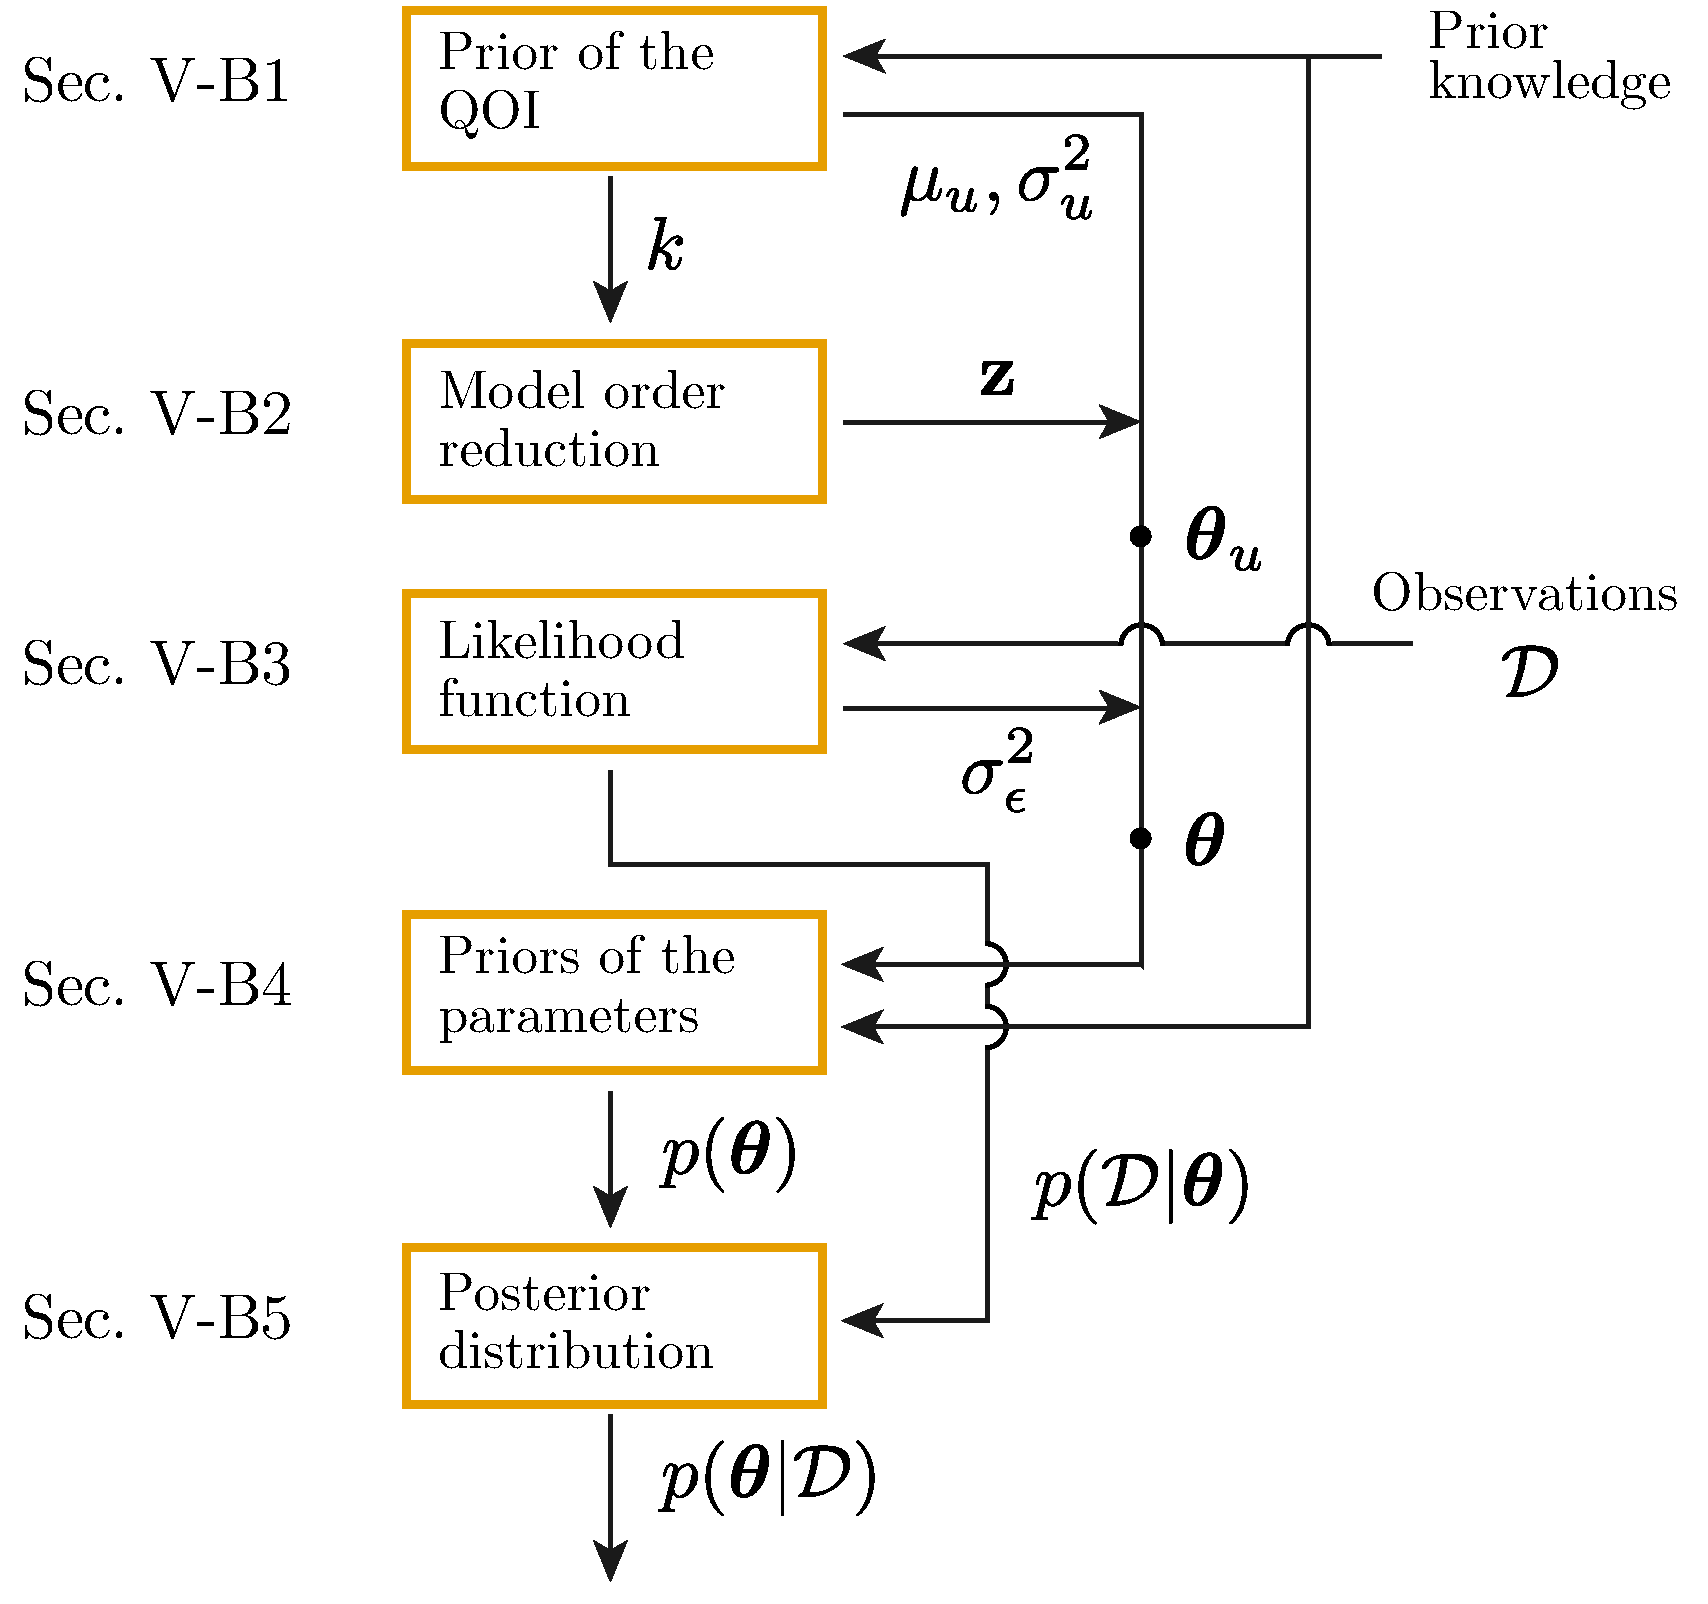
\includegraphics[width=1.0\linewidth]{include/figures/inference.pdf}
  \vspace{-0.7em}
  \caption{The statistical model.}
  \flabel{inference}
  \vspace{-1.3em}
\end{figure}

Since, at each point of the continuum of spatial locations on the wafer, the random element $\u$ can potentially take a different value, $\u$ is infinite-dimensional.
Hence, $\u$ can be seen as a stochastic process $\u(\o, \r)$, $\o \in \outcomes$, $\r \in \domain$, defined over a probability space with the set of outcomes $\outcomes$ \cite{durrett2010} and the spatial domain $\domain$ corresponding to the wafer.
Once the wafer has been fabricated, the probability space yields a particular outcome $\o$, and $\u$ becomes deterministic in the sense that it is fixed at each location, \ie, $\u(\o, \r) := \u(\r)$, $\r \in \domain$.
The values $\u(\r)$, $\r \in \domain$, however, are still unknown for us.
In order to infer them, we employ the procedure developed in the current subsection; we shall refer to this procedure as the statistical model, which is shown in \fref{algorithm} and detailed in \fref{inference}. This model closely follows the general Bayesian approach outlined in \sref{bayesian-inference} and consists of the five components described next.

\subsubsection{Modeling the \qoi}
The first step is to assign an adequate model to the unknown $\u$. We model $\u$ as a Gaussian process \cite{rasmussen2006} since (a) it is flexible in capturing the correlation patterns induced by the manufacturing process (described later on); (b) it is computationally efficient; and (c) Gaussian distributions are often natural and accurate models for uncertainties due to process variation \cite{srivastava2010, juan2011, juan2012}:
\[
  \u | \vparam_\u \sim \gaussianp{\fMean}{\fCov}
\]
where $\fMean$ and $\fCov$ are the mean and covariance functions of $\u$, respectively. Hereafter, the vertical bar, pronounced as ``given'', is used to mark the parameters that the probability distribution on the right-hand side depends on. In this case, such parameters are $\vparam_\u$, which we shall identify later on. Prior to taking any measurements, $\u$ is assumed to be spatially unbiased; therefore, we let $\fMean$ be a single location-independent parameter $\mu_\u$, \ie, $\fMean{r} = \mu_\u$, $\forall \r \in \domain$.
The covariance function $\fCov$ is chosen to be the following composition:
\begin{equation} \elabel{covariance-function}
  \fCov{\r, \r'} = \sigma_\u^2 \big( \eta \; \fCov_\SE(\r, \r') + (1 - \eta) \fCov_\OU(\r, \r') \big)
\end{equation}
where
\begin{align*}
  & \fCov_\SE(\r, \r') = \exp\left(-\frac{\norm{\r - \r'}^2}{\ell_\SE^2}\right) \text{ and} \\
  & \fCov_\OU(\r, \r') = \exp\left(- \frac{\abs{\,\norm{\r} - \norm{\r'}\,}}{\ell_\OU} \right)
\end{align*}
are the squared exponential and Ornstein-Uhlenbeck correlation functions, respectively; $\sigma_\u^2$ represents the variance of $\u$; $\eta \in [0, 1]$ is a weighting coefficient; $\ell_\SE$ and $\ell_\OU > 0$ are the length-scale parameters; and $\norm{\cdot}$ stands for the Euclidean distance.
The choice of the covariance function $\fCov$ is guided by the observations of the correlation structures induced by the fabrication process \cite{chandrakasan2001, cheng2011}: $\fCov_\SE$ imposes similarities between the points on the wafer that are close to each other, and $\fCov_\OU$ imposes similarities between points that are at the same distance from the center of the wafer.
The length-scale parameters $\ell_\SE$ and $\ell_\OU$ control the extend of these similarities, \ie, the range wherein the influence of one point on another is significant.
Although all the above parameters of the prior of $\u$ can be inferred from the data, for simplicity, we shall focus on $\mu_u$ and $\sigma_\u^2$.
The rest of the parameters, namely, $\eta$, $\ell_\SE$, and $\ell_\OU$ of the covariance function $\fCov$, are assumed to be determined \apriori\ to our analysis based on the knowledge of the correlation patterns typical for the production process utilized (see \cite{marzouk2009} and references therein).

\subsubsection{Model order reduction} \slabel{model-order-reduction}
The infinite-dimensional object $\u$ is reduced to a finite-dimensional one via the procedure described in \aref{kl-expansion}.
Specifically, we use \eref{covariance-function} to compute the covariance matrix of $\u$ with respect to the union of two sets of points on the wafer: the first one is composed of the $\nrdies \nrprocs$ spatial locations where the observations in $\Data$ were made (one location for each measured processing element on each of the selected dies), and the other of the locations where the user wishes to characterize $\u$.
For simplicity, we assume that the user is interested in all processing elements on all dies, which is $\ndies \nprocs$ locations in total (see \fref{wafer-measured}). Consequently, we obtain an $\ndies \nprocs$-dimensional representation of $\u$ denoted by the vector $\vu$. Then, following \aref{kl-expansion}, we factorize the computed covariance matrix and obtain the following decomposition of $\vu$:
\begin{equation} \elabel{kl-approximation}
  \vu = \mu_\u \vI + \sigma_\u \mKL \vz
\end{equation}
where we treat the constant multiplier $\sigma^2_\u$ in \eref{covariance-function} separately, $\vz = (\z_i) \in \real^\nvars$ obey the standard Gaussian distribution, and $\vI = (e_i = 1)$. The model order reduction procedure described in \aref{kl-expansion} is implied in \eref{kl-approximation}; thus, typically, $\nvars \ll \ndies \nprocs$. Let us define the identified parameters of the prior of $\u$ by $\vparam_\u = \{ \vz, \mu_\u, \sigma^2_\u \}$ (see \fref{inference}) and denote the forward model by $\mvT = \model{\vparam_\u}$.

\subsubsection{Likelihood function}
Due to the imperfection of the measurement process, the temperature profiles in $\Data$, stacked into $\mvT_\meas$, are assumed to deviate from the model prediction in \eref{model} for a given $\u$. To account for this,
\begin{equation} \elabel{noisy-measurements}
  \mvT_\meas = \model{\vparam_\u} + \vnoise = \mvT + \vnoise
\end{equation}
where $\vnoise$ is an $\nrdies \nrprocs \nrsteps$-dimensional vector of noise, which is typically assumed to be a white Gaussian noise \cite{rasmussen2006, marzouk2009}.
Without loss of generality, the noise is assumed to be independent of $\u$ and to have the same magnitude for all measurements (characterized by the utilized instruments). Therefore, the model of the noise is
\begin{equation} \elabel{noise-model}
  \vnoise | \sigma^2_\noise \sim \gaussian{0}{\sigma^2_\noise \mI}
\end{equation}
where $\sigma^2_\noise$ is a parameter defining the variance of the noise. Let us denote all the parameters identified so far by $\vparam = \vparam_\u \cup \{ \sigma_\noise^2 \} = \{ \vz, \mu_\u, \sigma_\u^2, \sigma_\noise^2 \}$ (see \fref{inference}).
Combining \eref{noisy-measurements} and \eref{noise-model}, we get
\begin{equation} \elabel{likelihood}
  \mvT_\meas | \vparam \sim \gaussian{\mvT}{\sigma_\noise^2 \mI}.
\end{equation}
The probability density function of this distribution is the likelihood function $\f{\Data | \vparam}$ of the data $\Data$.

\subsubsection{Priors of the parameters}
We put the following priors on $\vparam$:
\begin{align}
  & \z_i \sim \gaussian{0}{1}, \elabel{z-prior} \\
  & \mu_\u \sim \gaussian{\mu_0}{\sigma^2_0}, \elabel{mu-u-prior} \\
  & \sigma^2_\u \sim \sichisquared{\nu_\u}{\tau^2_\u}, \text{ and} \elabel{sigma2-u-prior} \\
  & \sigma^2_\noise \sim \sichisquared{\nu_\noise}{\tau^2_\noise}. \elabel{sigma2-noise-prior}
\end{align}
The prior for $\vz$ is due to the properties the decomposition in \eref{kl-approximation}.
The next three priors, \ie, a Gaussian and two scaled inverse chi-squared distributions, are a common choice for a Gaussian model with the mean and variance being unknown.
The parameters $\mu_0$, $\tau^2_\u$, and $\tau^2_\noise$ represent the presumable values of $\mu_u$, $\sigma^2_\u$, and $\sigma^2_\noise$, respectively, and are set by the user based on the prior knowledge on the technological process and measurement instruments employed. The parameters $\sigma_0$, $\nu_\u$, and $\nu_\noise$ reflect the precision of this prior information.
When the prior knowledge is weak, non-informative priors can be utilized \cite{gelman2004, bernardo2007}.
Taking the product of the density functions in \eref{z-prior}--\eref{sigma2-noise-prior}, we obtain the prior for all the parameters, denoted by $\f{\vparam}$ in \eref{bayes}.

\subsubsection{Posterior}
At this point, we have obtained the two pieces of the posterior shown in \eref{bayes}: the likelihood function, which is the density in \eref{likelihood}, and the prior, which is the product of the densities in \eref{z-prior}--\eref{sigma2-noise-prior}. Thus, the posterior reads as
\begin{equation} \elabel{posterior}
  \f{\vparam | \Data} \propto \f{\mvT_\meas | \vz, \mu_\u, \sigma^2_\u, \sigma^2_\noise} \; \f{\vz} \; \f{\mu_\u} \; \f{\sigma^2_\u} \; \f{\sigma^2_\noise}.
\end{equation}
This expression, given up to a constant multiplier, is sufficient for the Metropolis-Hastings algorithm (see \sref{bayesian-inference}). Therefore, assuming that we have an adequate proposal distribution (see the next subsection), we can readily draw samples from the posterior.
